\documentclass[10pt, conference]{IEEEtran}
\usepackage[english]{babel}
\usepackage[usenames]{color}
\usepackage{colortbl}
\usepackage{comment}
\usepackage{graphicx}
\usepackage{epsfig}
\usepackage{array, colortbl}
\usepackage{listings}
\usepackage{epstopdf}
\usepackage{multirow}
\usepackage{rotating}
%\usepackage{subfigure}
%\usepackage{subfig}
\usepackage{float}
\usepackage[obeyspaces,hyphens,spaces]{url}
\usepackage{balance}
\usepackage{fancybox}
\usepackage{scalefnt}
\usepackage[normalem]{ulem}
%\pagestyle{plain}
\pagenumbering{arabic}
\pagestyle{empty}
\clubpenalty = 10000
\widowpenalty = 10000
\displaywidowpenalty = 10000
\usepackage{cleveref}
\usepackage{latexsym}
\usepackage{amsfonts}
\usepackage{amssymb}

\usepackage{graphicx}
\usepackage{caption}
\usepackage{subcaption}


\makeatletter
\renewcommand{\paragraph}[1]{\noindent\textsf{#1}.}

\title{Scaling Databases with the Sharding Pattern on Amazon EC2}
\author{Zeinab Kermansaravi, Mohammed Sayagh
    \\
    \emph{zeinab.kermansaravi, mohammed.sayagh}@polymtl.ca}

\begin{document}
\maketitle

\begin{abstract}
\indent Database Sharding is a highly scalable approach for improving the throughput and overall performance of high-transaction, large database-centric business applications. Database Sharding is an excellent fit for many types of business applications, those with general purpose database requirements. It can also be used effectively for Data Warehousing applications, and there are many available products and technologies to accomplish this. In this lab, we implemented a distributed database architecture using the three strategies of Sharding pattern and also compare the performances between Sharding pattern and a simple MySql server. We found that MySql is better than MySql cluster when a request is simple and table structure is not complex, but the Sharding is better than MySql in the case where a request or a table structure are complexes. Therefore, implementing a sharding strategy is a better than MySql once a request is not executed only on one simple table (few columns). 

\end{abstract}

\section{Introduction}

\indent The concept of Database Sharding has been gaining popularity over the past several years, due to the enormous growth in transaction volume and size of business application databases. This is particularly true for many successful online service providers, Software as a Service (SaaS) companies, and social networking Web sites. Database Sharding can be simply defined as a "shared-nothing" partitioning scheme for large databases across a number of servers, enabling new levels of database performance and scalability achievable. \\
\indent The term "sharding" was coined by Google engineers, and popularized through their publication of the Big Table architecture. However, the concept of “shared-nothing” database partitioning has been around for a decade or more and there have been many implementations over this period, especially high profile in-house built solutions by Internet leaders such as eBay, Amazon, Digg, Flickr, Skype, YouTube, Facebook, Friendster, and Wikipedia.\\
\indent The idea behind sharding is to split data among multiple machines while ensuring that the data is always accessed from the correct place. Since sharding spreads the database across multiple machines, the database programmer specifies explicit sharding rules to determine which machines any piece of data will be stored on.\\
\indent This lab perform scaling databases with sharding pattern on Amazon EC2. To reach this goal, we installed and run MySQL and MySQL cluster on Amazon EC2, got the results and compared them. Then, we implement three sharding strategy to distribute the data in Sakila database and compared the results of each strategy and Finally we have a solution, analysis and disscussion on these strategies. 


\section{Background}
\indent In this section, we have an introduction of MySQL Cluster, then we explain what the design patterns are? and how they are used in clouds, then, we introduce Sysbench, we also describe the sharding pattern which is one of the types of design patterns. And finally, we introduce three common strategies which used to distribute data in to a set of shards on Amazon EC2.
\subsection{MySQL Cluster}
\indent MySQL Cluster is a technology that enables clustering of in-memory databases in a shared-nothing system, in which, the shared-nothing architecture enables the system to work with very inexpensive hardware, and with a minimum of specific requirements for hardware or software. In a shared-nothing system, each component is expected to have its own memory and disk, and the use of shared storage mechanisms such as network shares, network file systems, and SANs is not recommended or supported. In this case, MySQL Cluster integrates the standard MySQL server with an in-memory clustered storage engine called NDB (which stands for "Network DataBase"). It should be noted that, NDB refers to the part of the setup that is specific to the storage engine, whereas "MySQL Cluster" refers to the combination of one or more MySQL servers with the NDB storage engine. A MySQL Cluster consists of a set of computers ("hosts"), each running one or more processes which called "nodes". Nodes, may include MySQL servers (for access to NDB data), data nodes (for storage of the data), one or more management servers, and possibly other specialized data access programs. The relationship of these components in a MySQL Cluster shows in figure 1. 

\begin{figure}[h!]
	\centering
	\includegraphics[width=9cm]{figure1.jpg}
	\caption{MySQL Cluster Structure[1]}
\end{figure} 
\indent All these programs work together to form a MySQL Cluster. When data is stored by the NDB storage engine, the tables (and table data) are stored in the data nodes. Such tables are directly accessible from all other MySQL servers (SQL nodes) in the cluster. Thus, in a payroll application storing data in a cluster, if one application updates the salary of an employee, all other MySQL servers that query this data can see this change immediately. However, a MySQL server that is not connected to a MySQL Cluster cannot use the NDB storage engine and cannot access any MySQL Cluster data [1].

\subsection{Sysbench}
\indent Sysbench is a popular open source benchmark to test open source DBMSs. More completely, SysBench is a modular, cross-platform and multi-threaded benchmark tool for evaluating OS parameters that are important for a system running database under intensive load. The idea of this benchmark suite is to quickly get an impression about system performance without setting up complex database benchmarks or even without installing a database at all. Current features allow to test the following system parameters:

\begin{itemize}
\item file I/O performance
\item scheduler performance
\item memory allocation and transfer speed
\item POSIX threads implementation performance
\item database server performance.
\end{itemize}

\indent Available test modes are implemented by compiled-in modules, and SysBench was designed to make adding new test modes an easy task. Each test mode may have additional (or workload-specific) following options:
\begin{itemize}
\item --num-threads: The total number of worker threads to create (defaut: 1)
\item --max-requests: Limit for total number of requests. 0 means unlimited (defaut 10000)
\item --max-time: Limit for total execution time in seconds. 0 (defaut: 0)
\item --thread-stack-size: Size of stack for each thread (defaut: 32K)
\item --init-rnd: Specifies if random numbers generator should be initialized from timer before the test start (defaut: off)
\item --test: Name of the test mode to run Required
\item --debug: Print more debug info (default: off)
\item --validate: Perform validation of test results where possible (default: off)
\item --help: Print help on general syntax or on a test mode specified with --test, and exit
\item --version: Show version of program.
\item --percentile: SysBench measures execution times for all processed requests to display statistical information like minimal, average and maximum execution time. For most benchmarks it is also useful to know a request execution time value matching some percentile (e.g. 95% percentile means we should drop 5% of the most long requests and choose the maximal value from the remaining ones). This option allows to specify a percentile rank of query execution  times to count (default: 95)
\item --batch: Dump current results periodically (default: off )
\item --batch-delay: Delay between batch dumps in secods (default: 300) Note that numerical values for all size options (like --thread-stack-size in this table) may be specified by appending the corresponding multiplicative suffix (K for kilobytes, M for megabytes, G for gigabytes and T for terabytes).
\end{itemize}

\subsection{Design Patterns}
\indent In general, Design pattern is defined as a general good and reuseable solution to a commonly occuring problem. A design pattern is known using some major elements includes:

\begin{itemize}
\item a Name for the Design Pattern;
\item a description or a model to be applied to solve a problem that can occur in different situations during the design process;
\item a problem, or the description of the situation you can apply the pattern to;
\item a solution describing the elements of the project with the relations and their consequences;
\item the consequences, results and constraints resulting from the application of the pattern.
\end{itemize}

\indent But, in AWS Cloud Design Patterns, there is a bit difference in the general definition which is "AWS Cloud Design Patterns are a collection of solutions and design ideas aimed at using the AWS Cloud technology to solve common systems design problems", so, in this case, a Cloud Design Pattern might be described as follows:

\begin{itemize}
\item Pattern Name/Summary: Pattern name, summary and brief description;
\item Solving Issues: Description of typical issues that led to pattern creation, and what issues/challenges can be solved through its implementation;
\item Explanation of pattern / Resolution in the cloud: Description of the terms or how to solve the problems in the cloud; why any pattern, or a description of the configuration has become a pattern of what;
\item Implementation: Description about how to implement the pattern using AWS;
\item Benefits: Description of the benefits from the pattern’s application;
\item Notes: Description of tradeoffs, advantages, disadvantages and points to note when applying this pattern;
\item Other: Comparison with other patterns, use cases and additional information.
\end{itemize}

\indent Design patterns are helpful because they represent field-tested solutions to common design problems, organize design intelligence into a standardized and easily referenced format. They are generally repeatable by most IT professionals involved with design, they can be used to ensure consistency in how systems are designed and built and also can become the basis for design standards. They are usually flexible and optional (and openly document the impacts of their application and even suggest alternative approaches). Besides, they can be used as educational aids by documenting specific aspects of system design (regardless of whether they are applied), they can sometimes be applied prior and subsequent to the implementation of a system. Disign patterns can be supported via the application of other design patterns that are part of the same collection, and enrich the vocabulary of a given IT field because each pattern is given a meaningful name as well. Furthermore, because the solutions provided by design patterns are proven, their consistent application tends to naturally improve the quality of system designs. But, it is important to note that, even though design patterns provide proven design solutions, their mere use cannot guarantee that design problems are always solved as required. Many factors weigh in to the ultimate success of using a design pattern, including constraints imposed by the implementation environment, competency of the practitioners, diverging business requirements, and so on. All of these represent aspects that affect the extent to which a pattern can be successfully applied [2]. \\
\indent There are several types of design patterns, for example, some of them which mentioned in Mcrosoft website [3] are: Cache-aside Pattern, Circuit Breaker Pattern, Compensating Transaction Pattern, Competing Consumers Pattern, Compute Resource Consolidation Pattern, Command and Query Responsibility Segregation (CQRS) Pattern, Event Sourcing Pattern, External Configuration Store Pattern, Federated Identity Pattern, Gatekeeper Pattern, Health Endpoint Monitoring Pattern, Index Table Pattern, Leader Election Pattern, Materialized View Pattern, Pipes and Filters Pattern, Priority Queue Pattern, Queue-based Load Leveling Pattern, Retry Pattern, Runtime Reconfiguration Pattern, Scheduler Agent Supervisor Pattern, Sharding Pattern, Static Content Hosting Pattern, Throttling Pattern, Valet Key Pattern.
 
\subsection{Sharding Pattern}
\indent Sharding pattern is used to divide (shard) a data store into a set of horizontal partitions or shards. Each shard has the same schema as the original database, but holds its own distinct subset of the data. A shard is a data store in its own right (it can contain the data for many entities of different types), running on a server acting as a storage node. Most data is distributed such that each row appears in exactly one shard. The combined data from all shards is the same as the data from the original database. This pattern can improve scalability when storing and accessing large volumes of data. This pattern offers the following benefits:
\begin{itemize}
\item You can scale the system out by adding further shards running on additional storage nodes.
\item A system can use off the shelf commodity hardware rather than specialized (and expensive) computers for each storage node.
\item You can reduce contention and improved performance by balancing the workload across shards.
\item In the cloud, shards can be located physically close to the users that will access the data.
\end{itemize}
\indent When dividing a data store up into shards, decide which data should be placed in each shard. A shard typically contains items that fall within a specified range determined by one or more attributes of the data. These attributes form the shard key (sometimes referred to as the partition key). The shard key should be static. It should not be based on data that might change. Sharding physically organizes the data.\\
\indent  When an application stores and retrieves data, the sharding logic directs the application to the appropriate shard. This sharding logic may be implemented as part of the data access code in the application, or it could be implemented by the data storage system if it transparently supports sharding. Abstracting the physical location of the data in the sharding logic provides a high level of control over which shards contain which data, and enables data to migrate between shards without reworking the business logic of an application should the data in the shards need to be redistributed later (for example, if the shards become unbalanced).\\
\indent The tradeoff is the additional data access overhead required in determining the location of each data item as it is retrieved. To ensure optimal performance and scalability, it is important to split the data in a way that is appropriate for the types of queries the application performs. In many cases, it is unlikely that the sharding scheme will exactly match the requirements of every query. For example, in a multi-tenant system an application may need to retrieve tenant data by using the tenant ID, but it may also need to look up this data based on some other attribute such as the tenant’s name or location. To handle these situations, implement a sharding strategy with a shard key that supports the most commonly performed queries. If queries regularly retrieve data by using a combination of attribute values, it may be possible to define a composite shard key by concatenating attributes together. Alternatively, use a pattern such as Index Table to provide fast lookup to data based on attributes that are not covered by the shard key.\\
\indent Three strategies are commonly used when selecting the shard key and deciding how to distribute data across shards. Note that there does not have to be a one-to-one correspondence between shards and the servers that host them—a single server can host multiple shards. The strategies are:
\begin{itemize}
\item The Lookup strategy
\item The Range strategy
\item The Hash strategy
\end{itemize}

\subsubsection{The Lookup strategy}
\indent  In this strategy the sharding logic implements a map that routes a request for data to the shard that contains that data by using the shard key. In a multi-tenant application all the data for a tenant might be stored together in a shard by using the tenant ID as the shard key. Multiple tenants might share the same shard, but the data for a single tenant will not be spread across multiple shards. Figure 2 shows an example of this strategy. \\
\begin{figure}[h!]
	\centering
	\includegraphics[width=9cm]{figure2.jpg}
	\caption{Sharding tenant data based on tenant IDs[3]}
\end{figure} 
\indent The mapping between the shard key and the physical storage may be based on physical shards where each shard key maps to a physical partition. Alternatively, a technique that provides more flexibility when rebalancing shards is to use a virtual partitioning approach where shard keys map to the same number of virtual shards, which in turn map to fewer physical partitions. In this approach, an application locates data by using a shard key that refers to a virtual shard, and the system transparently maps virtual shards to physical partitions. The mapping between a virtual shard and a physical partition can change without requiring the application code to be modified to use a different set of shard keys.\\
\indent Advantages: This strategy has more control over the way that shards are configured and used. Besides, using virtual shards reduces the impact when rebalancing data because new physical partitions can be added to even out the workload. The mapping between a virtual shard and the physical partitions that implement the shard can be modified without affecting application code that uses a shard key to store and retrieve data.\\
\indent But, it should be noted that, looking up shard locations can impose an additional overhead.

\subsubsection{The Range strategy}
\indent This strategy groups related items together in the same shard, and orders them by shard key—the shard keys are sequential. It is useful for applications that frequently retrieve sets of items by using range queries (queries that return a set of data items for a shard key that falls within a given range). For example, if an application regularly needs to find all orders placed in a given month, this data can be retrieved more quickly if all orders for a month are stored in date and time order in the same shard. If each order was stored in a different shard, they would have to be fetched individually by performing a large number of point queries (queries that return a single data item). Figure 3 shows an example of this strategy.\\
\begin{figure}[h!]
	\centering
	\includegraphics[width=9cm]{figure3.jpg}
	\caption{Storing sequential sets (ranges) of data in shards[3]}
\end{figure} 
\indent In this example, the shard key is a composite key comprising the order month as the most significant element, followed by the order day and the time. The data for orders is naturally sorted when new orders are created and appended to a shard. Some data stores support two-part shard keys comprising a partition key element that identifies the shard and a row key that uniquely identifies an item within the shard. Data is usually held in row key order within the shard. Items that are subject to range queries and need to be grouped together can use a shard key that has the same value for the partition key but a unique value for the row key.\\
\indent Advantages: This strategy is easy to implement and works well with range queries because they can often fetch multiple data items from a single shard in a single operation. It has also easier data management. For example, if users in the same region are in the same shard, updates can be scheduled in each time zone based on the local load and demand pattern.\\
\indent But, this strategy, may not provide optimal balancing between shards. Moreover, rebalancing shards is difficult and may not resolve the problem of uneven load if the majority of activity is for adjacent shard keys. 

\subsubsection{The Hash strategy}
\indent The purpose of this strategy is to reduce the chance of hotspots in the data. It aims to distribute the data across the shards in a way that achieves a balance between the size of each shard and the average load that each shard will encounter. The sharding logic computes the shard in which to store an item based on a hash of one or more attributes of the data. The chosen hashing function should distribute data evenly across the shards, possibly by introducing some random element into the computation. Figure 4 shows an example of this strategy.\\
\begin{figure}[h!]
	\centering
	\includegraphics[width=9cm]{figure4.jpg}
	\caption{Sharding tenant data based on a hash of tenant IDs[3]}
\end{figure} 
\indent To understand the advantage of the Hash strategy over other sharding strategies, consider how a multi-tenant application that enrolls new tenants sequentially might assign the tenants to shards in the data store. When using the Range strategy, the data for tenants 1 to n will all be stored in shard A, the data for tenants n+1 to m will all be stored in shard B, and so on. If the most recently registered tenants are also the most active, most data activity will occur in a small number of shards—which could cause hotspots. In contrast, the Hash strategy allocates tenants to shards based on a hash of their tenant ID. This means that sequential tenants are most likely to be allocated to different shards which will distribute the load across these shards.\\
\indent Advantages: It has better chance of a more even data and load distribution. Also, request routing can be accomplished directly by using the hash function. There is no need to maintain a map.\\
\indent But, computing the hash may impose an additional overhead and also, rebalancing shards is difficult.\\

\indent Each of the sharding strategies implies different capabilities and levels of complexity for managing scale in, scale out, data movement, and maintaining state.
\begin{itemize}
\item The Lookup strategy permits scaling and data movement operations to be carried out at the user level, either online or offline. The technique is to suspend some or all user activity (perhaps during off-peak periods), move the data to the new virtual partition or physical shard, change the mappings, invalidate or refresh any caches that hold this data, and then allow user activity to resume. Often this type of operation can be centrally managed. The Lookup strategy requires state to be highly cacheable and replica friendly.
\item The Range strategy imposes some limitations on scaling and data movement operations, which must typically be carried out when a part or all of the data store is offline because the data must be split and merged across the shards. Moving the data to rebalance shards may not resolve the problem of uneven load if the majority of activity is for adjacent shard keys or data identifiers that are within the same range. The Range strategy may also require some state to be maintained in order to map ranges to the physical partitions.
\item The Hash strategy makes scaling and data movement operations more complex because the partition keys are hashes of the shard keys or data identifiers. The new location of each shard must be determined from the hash function, or the function modified to provide the correct mappings. However, the Hash strategy does not require maintenance of state.
\end{itemize}

\section{Approach - Results - Discussion}

In this section, we provide the results of each one of the three experiences we performed. We present for each one its approach, the results, and discussion of the results.

\subsection{Benchmarking MySQL and MySQL Cluster}

\subsubsection{Approach} 

\indent We used Sysbench to compare between MySQL and MySQL Cluster performance.

\indent For the first experiments, we used Sysbench to compare between MySQL and MySQL Cluster performance. For this part, first of all, we created a t2.micro instance, we installed MySQL and Sysbench on this intance. One of the parameters in Sysnbench is "host" which specifies the MySQL server IP. To analyse the performance of MySQL, Sysbench create a table in a database, which we manually created. The created table is used to benchmark MySQL.
\begin{figure}[h!]
	\centering
	\includegraphics[width=9cm]{figure5.jpg}
\end{figure} 
\indent This command has two different statement includes "prepare" and "run". Prepare is used when we want to generate a table in the specified database which will be used when performing test and run is used when we want to evaluate the performances of a database server.\\
\indent Then, we have to do the same steps on MySQL Cluster to get results and compare these two bunchs of the results which shows the differences in performance of these two database servers (MySql and MySql cluster). In this step, we created six instances which are also t2.micro instances, so, we had four data nodes, one management node and one SQL node which we apply requests on. We have to notify that the number of replication was equal to one, which means that there is no backup for any data node, since we do not need in this Lab any backup evaluation, and therefore the four data nodes contains different data. We installed Sysbench on a seventh instance (Client instance) and we created a database (database sbtest) for testing in sql node, then we did the query on like the following commands: \\
\begin{figure}[h!]
	\centering
	\includegraphics[width=9cm]{figure6.jpg}
\end{figure}
\indent As you can see in two previous command, the parameter "mysql-table-engine" has a different value, which has a "innodb" value when it is MySQL and has a "ndbcluster" value when it is MySQL Cluster. Moreover, we changed the IP adress, which is MySql server when the tests are on MySql, and the IP adress of Sql Node where the tests are on MySql cluster.

To install and configure MySql cluster, we used the instructions provided in \cite{MySQLCluster}, which we adapted and modified by referring to the instruction of \cite{MySQLCluster2}, especially in the case where we have to add new data nodes. 

While we can not install Sql node and Sysbench in one instance, we installed Sysbench in another instance. Moreover, to overcome that the networking time impacts the benchmarking results, we performed the benchmarking of the MySql performances from another instance than the instance where MySql benchmarked is installed.

\begin{figure}[h!]
	\centering
	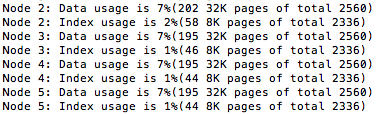
\includegraphics[width=9cm]{MemoryUsage.png}
	\caption{MySql Cluster memory usage}
	\label{fig:MemoryUsage}
\end{figure} 

To make sure that MySql Cluster well splits data between the four data nodes, we executed the following command in MySql Cluster: ALL REPORT MemoryUsage. And we found that MySql Cluster well dispatched data between the different data nodes, as highlighted by Figure \ref{fig:MemoryUsage}.

\begin{figure}[h!]
	\centering
	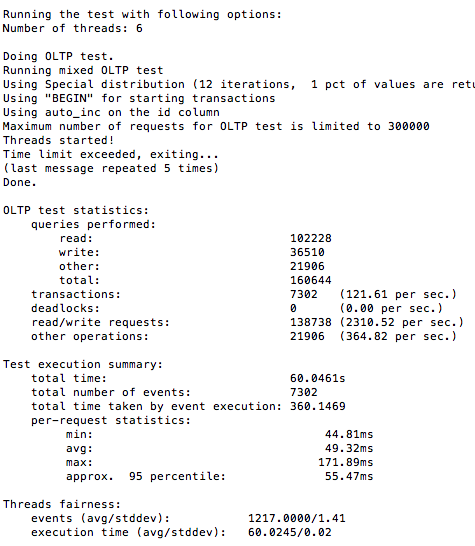
\includegraphics[width=9cm]{results1.png}
	\caption{MySql benchmarking performances}
	\label{fig:results1}
\end{figure} 


\subsubsection{Results} We found that MySql performs 160644 queries in 60 seconds, where 102228 are read queries, 36510 write queries, and 21906 other queries. Moreover, the minimum time of each request is 43.81ms, the average is 49.32ms, whereas the maximum time is 171.89ms. Figure \ref{fig:results1} shows more detail about the results of benchmarking performances for MySQL.

\begin{figure}[h!]
	\centering
	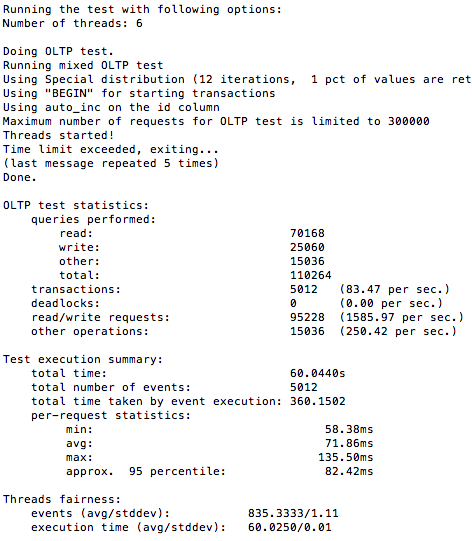
\includegraphics[width=9cm]{results2.png}
	\caption{MySql Cluster benchmarking performances}
	\label{fig:results2}
\end{figure} 

Benchmarking MySql Cluster using one management node, four data nodes, and one sql node provides a total of 110264 queries in 60 seconds, where 70168 ones are read operations, 25060 writes operations, and 15036 other operations. Figure \ref{fig:results2} provides more details about the results of benchmarking MySql cluster.


\begin{figure}[h!]
	\centering
	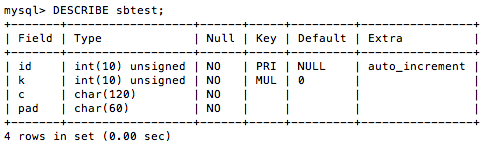
\includegraphics[width=9cm]{sbtestStructure.png}
	\caption{Structure of the test table used by Sysbench benchmark}
	\label{fig:sbtestStructure}
\end{figure} 

\subsubsection{Discussion} We observe that MySql provides more queries in 60 seconds than MySql cluster. We refer this differences to the fact that Sysbench analyzes the performance of a database by installing only one table, which makes the requests sent by Sysbench to MySql or MySql cluster server not complex and hence not time consuming. Moreover, as Figure \ref{fig:sbtestStructure} provides, the structure of this table is not complex, and moreover, it contains an index (id) which mainly can reduce a request time.

Therefore, we can say that MySql is better than MySql Cluster where the table structure is not complex and the queries are not complexes, which we also prove in Section \ref{section:Benchmarking sharding}.

\subsection{Implementing the sharding patterns}

\subsubsection{Approach} We used Hibernate shards in order to implement the sharding pattern strategies. To implement the sharding strategies, we used maven to download the dependencies we need, and we created a hibernate configuration file for each shard (all the hibernate configuration files are stored in resources of the project available on Git). 

While we used Sakila as a case study, we used JPA to create the mapping annotations between sakila tables and the Java model, which we manually refined, especially by modifying the cascade operations (updates and inserts). We also used the option "fetch" to read the attributes related to an object, for example to read the actors related to a film once we read a film from the database. Moreover, we adequately placed fetch in the right places to load data that we have to dispatch between our four shards, in order to do not forget any element in the whole sakila database. 

One of the main element of the sharding pattern strategies is to choose the right shard where to write data or from where to read data. We created a method that has to return the shard id, the method should be in a Class implementing our interface "ShardingStrategy", this Class represents the sharding strategy, we developed a class for the lookup strategy (Util.LookupStrategy.java), another class for the range strategy (Util.RangeStrategy.java), and a third class for hash strategy (Util.HashStrategy.java). These classes are injected into a class that insert and read data from different shards (ConnexionTest.DAO.java).

For the sharding table, we choose a table that represents a root table, which is the table "category". For the lookup strategy, we used the modulo of the category id divided by 4 (the number of instances). For the range strategy, we put from the first to the fourth categories in the first shard, from the fifth to the eighth categories in the second shard, from the ninth to the twelfth categories in the third shard, and from the thirteenth to the sixteenth categories in the fourth shard. For the hash strategy, we implemented the method hashCode for the class Category, we used this hash method, which we computed its modulo of its division by 4, to choose which shard contains which data, and in which shard we have to write an instance.

We also created four t2.micro instances, where we installed in each one MySql server. 

To evaluate how our sharding implementation is efficient, we computed the size of each node after the sharding execution, by executing the following command:

"SELECT table\_schema                                        DB\_Name,     Round(Sum(data\_length + index\_length) / 1024 / 1024, 1) "DB Size in MB"  FROM   information\_schema.tables  where table\_schema = "sakila1" GROUP  BY table\_schema;" 

The sources code are available on Git repository.



\begin{figure}
	\centering
	\begin{subfigure}[b]{0.33\textwidth}
	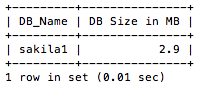
\includegraphics[width=6cm]{size1.png}
	\caption{Shard 1 database size}
	\end{subfigure}
	\begin{subfigure}[b]{0.33\textwidth}
		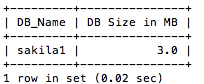
\includegraphics[width=6cm]{size2.png}
		\caption{Shards 2 and 3 databases size}
	\end{subfigure}
	\begin{subfigure}[b]{0.33\textwidth}
		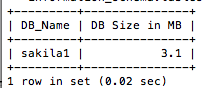
\includegraphics[width=6cm]{size3.png}
		\caption{Shard 4 database size}
	\end{subfigure}
	\caption{The size of the database of each shard.}
	\label{fig:sizeShards}
\end{figure} 


\subsubsection{Results} By dividing data using our implementation of the three strategies, we found that the data is well splited between the four nodes, where each one contains a size higher between 2.9 MB and 3.1 MB, while the whole database of sakila contains 8.1 MB. Figure \ref{fig:sizeShards} highlights the size of each database shard. we refer to the difference between the sum of shards size and sakila size to the fact that only the structure of sakila contains 0.7MB. Therefore, the sharding is efficient.

The results are the same for the three sharding strategies.

\subsection{Benchmarking the sharding implementation}
\label{section:Benchmarking sharding}

\subsubsection{Approach} To evaluate our implementation, we compare the execution time between two same requests, while the first one is executed in the whole sakila database, the second one is executed in the sharding nodes. 

To evaluate when the sharding pattern provides more important performance than a simple MySql server, we use different requests, from the less complex requests (request on one table) to the more complex requests (queries joining 5 tables). 

We should notify that the results for the three implementations gives approximately the same performances.


	\begin{table*}
		\begin{center}
			\begin{tabular}{|l|l|l|l|}
				\hline
				Number of tables & The tables in join request & MySql (ms) & Sharding implementation (ms) \\
				\hline
				1 & Category & 190 & 194 \\
				4 & Category, Film, Film\_category, Language  & 1074 & 854 \\
				5 & Category, Film, Film\_category, Language, inventory & 4846 & 2236 \\
				\hline
			\end{tabular}
			\caption{\label{executiontime} Difference between MySql and MySql with Sharding pattern execution time.}
		\end{center}
	\end{table*}

\subsubsection{Results} Table \ref{executiontime} provides the execution time between the time needed to provide the results of a query using the whole sakila database installed in one server, and the implementation of the sharding pattern. A query on one table (the table Category) needs 190 ms to return results from MySql server, where it needs 194 ms using the sharding implementation. Moreover, a query on four joined tables is executed in 1074 ms using Sakila installed in only one MySql server, whereas it needs 854 ms using Sakila installed in four servers and using the sharding implementation. Furthermore, a query on five joined tables is executed in 4846 ms in MySql, whereas only 2236 ms in four MySql servers and using the sharding implementation. 

\subsubsection{Discussion} We observe from the results that more requests are complexes, more sharding provides results faster than a simple MySql. Therefore, the sharding is more important when requests are complexes. Because, the complex requests are less time consuming when data size is not high (the shards case). 

We also observe that when we added a fifth table (the table inventory), we get an important difference between MySql and MySql using sharding pattern, to understand this result, we analyzed data stored in the table "inventory". And we found that Sakila contains around 4000 elements in this table, and by splitting data using sharding pattern, the table "inventory" contains only around 1000 elements in each shard, which makes the request on MySql more time consuming than the requests on MySql Shards using one of the sharding strategies. 

While a request is complex, and the tables participating in this request contains an important number of occurrences, the sharding pattern provides results in lower time than the requests on a simple MySql server. Moreover, MySql is more efficient than MySql Clusters when a query is not complex and there are not a lot of data, which explains more the results obtained by Sysbench in the first experiment.

\section{conclusion}
\indent Database systems with large data sets and high throughput applications can challenge the capacity of a single server. To solve such problems, sharding concept has been emerged which is a database scalability technique that has proven itself in some of the world’s most popular MySQL web sites, applications and games. This work implemented a distributed database architecture using sharding pattern. Two different database sever includes MySQL and MySQL Cluster has been installed and their performance have been compared using Sysbench benchmark. The results shows that dividing data in different shards provide higher performances than a simple MySql server for the three sharding strategies. The results also provide that while a request is more complex and more a table participating in the request contains more data, Sharding provides results in lower time than a simple MySql server. While in the majority of real life cases, sql requests contain a least two tables, sharding data becomes efficient than a simple MySql. Therefore, we conclude that sharding data in many servers is better than using only one MySql server, independently on the sharding strategy.


\balance
\bibliographystyle{IEEEtran}
\bibliography{assignment.bib}



\end{document}
